\documentclass[conference]{IEEEtran}
\IEEEoverridecommandlockouts
% The preceding line is only needed to identify funding in the first footnote. If that is unneeded, please comment it out.
\usepackage{cite}
\usepackage[ngerman]{babel}
\usepackage[utf8]{inputenc}
\usepackage{amsmath,amssymb,amsfonts}
\usepackage{algorithmic}
\usepackage{graphicx}
\usepackage{textcomp}
\usepackage{xcolor}
\usepackage{listings}


\definecolor{pblue}{rgb}{0.13,0.13,1}
\definecolor{pgreen}{rgb}{0,0.5,0}
\definecolor{pred}{rgb}{0.9,0,0}
\definecolor{pgrey}{rgb}{0.46,0.45,0.48}
\lstset{language=Python,
	showspaces=false,
	showtabs=false,
	breaklines=true,
	tabsize=2,
	showstringspaces=false,
	breakatwhitespace=true,
	commentstyle=\color{pgreen},
	keywordstyle=\color{pblue},
	stringstyle=\color{pred},
	basicstyle=\ttfamily
}


\usepackage{url}
\def\BibTeX{{\rm B\kern-.05em{\sc i\kern-.025em b}\kern-.08em
		T\kern-.1667em\lower.7ex\hbox{E}\kern-.125emX}}
\begin{document}
	
	\title{Videoanalyse und Objekttracking}
	
	\author{\IEEEauthorblockN{1\textsuperscript{st} Bartolovic Eduard}
	\IEEEauthorblockA{\textit{Hochschule München} \\
		München, Deutschland \\
		eduard.bartolovic0@hm.edu}
	\and
	\IEEEauthorblockN{2\textsuperscript{nd} Thomas Willeit}
	\IEEEauthorblockA{\textit{Hochschule München} \\
		München, Deutschland \\
		XXXXX@hm.edu}
	\and
	\IEEEauthorblockN{3\textsuperscript{rd} Schäfer Julia}
	\IEEEauthorblockA{\textit{Hochschule München} \\
		München, Deutschland \\
		j.schaefer0@hm.edu}
	}

	
	\maketitle
	
	\begin{abstract}
		
	\end{abstract}
	
	\section{Konzept}
	Ziel des Projektes ist es klassische Verfahren mit neuere DeepLearning Verfahren zu vergleichen.
	Dafür ist für beide arten eine Pipeline geschaffen worden.\\
	Für die Klassische Verfahren wurde für die Objekterkennung Gausmixture verwendet und für das Tracking Sort. Für die DeepLearnig Verfahren wurde für die Objekterkennung ein Neuronales Netz  und für das Tracking wurde Deepsort verwendet.
	
	\begin{figure}[h]
		\begin{center}
			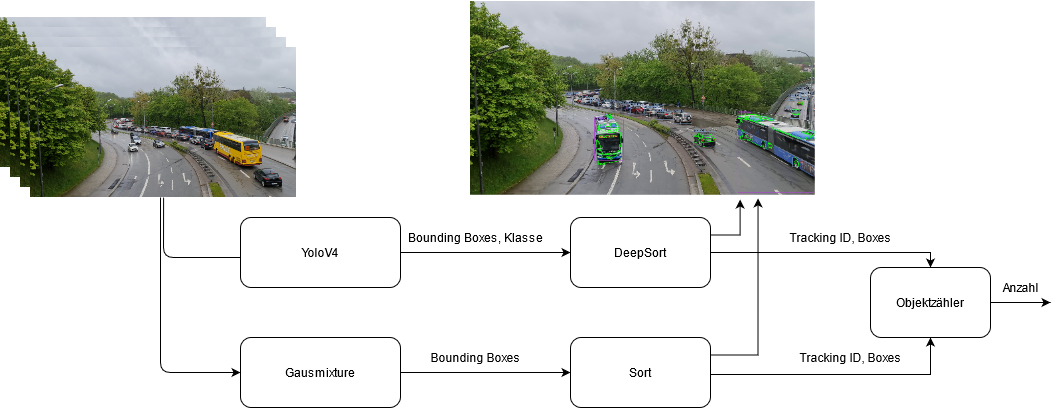
\includegraphics[width=14cm]{Media/KonzeptVAOT.png}
			\caption{Konzept für das Projekt}
			\label{Konzept}
		\end{center}
	\end{figure}
	
	\section{Objekterkennung: Gauß Mixture}
	
	\section{Objekterkennung: YoloV4}
	YOLO ist ein Neuronal Netz für die Echtzeit-Objekterkennung. YOLO ist die Abkürzung für 'You Only Look Once' was übersetzt 'Man sieht nur einmal hin' heißt. Die Aufgabe der Objekterkennung besteht darin, den Ort und die Boundingbox im Bild zu bestimmen, sowie die Objekte zu klassifizieren. Frühere Methoden, wie R-CNN und seine Variationen, verwendeten eine Pipeline, um diese Aufgabe in mehreren Schritten durchzuführen. Dies ist in der Ausführung langsam und aufwendiger zu trainieren, da jede einzelne Komponente separat trainiert werden muss. YOLO, erledigt beide Aufgaben mit einem einzigen neuronalen Netzwerk. Es betrachtet dabei die Objekterkennung als ein Regressionsproblem auf räumlich getrennte Bounding Boxes und zugehörige Klassenwahrscheinlichkeiten.\cite{b1}\\
	Das Bild in ein S × S-Gitter mit den Residualblöcken aufgeteilt. Wenn der Mittelpunkt eines Objekts in eine Gitterzelle fällt, ist diese Gitterzelle für die Erkennung dieses Objekts zuständig. Jede Gitterzelle sagt B Bounding Boxes und C Klassen Konfidenzwerte für diese Boxen voraus \cite{b1}\\
	Diese Klassen Konfidenzwerte zeigen, wie sicher das Modell ist, dass die Boundingbox ein Objekt enthält und auch wie genau die Box das Objekt beschreibt. Die Konfidenz wird wie folgt definiert:
	\[ c = Pr(Objekt) * IOU_{pred}^{truth} \]
	Jede Boundingbox enthält die 5 Vorhersagen: x,y,w,h,c.
	Jede Gitterzelle sagt auch bedingte Klassenwahrscheinlichkeiten $Pr(Class_{i}|Object)$, voraus.  Diese Wahrscheinlichkeiten beziehen sich auf die Gitterzelle, die ein Objekt enthält.
	Zum Testzeitpunkt wird die bedingten Klassenwahrscheinlichkeiten und die individuellen Box-Vertrauensvorhersagen multipliziert, wodurch wir klassenspezifische Vertrauenswerte für jede Box erhalten.  Diese Werte kodieren sowohl die Wahrscheinlichkeit, dass diese Klasse in der Box vorkommt, als auch, wie gut die vorhergesagte Box zum Objekt passt.
	\[ Pr(Class_{i}|Object)*Pr(Object)*IOU_{truth}^{pred}= Pr(Class_{i})*IOU_{truth}^{pred} \]
	........Netzwerk???...........
	........LossFunction???...........
	
	Da Objekte meist immer ähnliche Formen haben kann man eine gewisse Menge an sogenannten Ankerboxen definieren welche als Basis Boundingboxen fingieren. Diese Ankerboxen kann man mittels Clusteralgorithmen wie K-Means und den Boundingboxen aus dem Datensatz berechnen....\\
	In diesem Projekt verwendeten wir die 4te und damit aktuell neueste Version von Yolo\cite{b2}. So bietet jede Version inkrementelle Verbesserung zum jeweiligen Vorgänger.\\
	Unser Modell wurde bereits mit dem Microsoft COCO Datensatz trainiert. Es sind 80 verschiedene Klassen erkennbar. Wir interessieren uns aber nur für einen kleineren Teil wie:
	\begin{enumerate}
		\item Personen
		\item Pkw
		\item Lkw
		\item Busse
		\item Fahrräder
		\item Züge
	\end{enumerate}
	Je nach Szenario lassen sich per Parameter die relevanten Klassen auswählen. Das Modell prädiktiert trotzdem noch alle Klassen. Die nicht relevanten werden einfach im Postprocessing herausgefiltert. Das Ergebnis einer Prädiktion ist eine Liste von Objekten welches aus den x,y Koordinate des Mittelpunktes der Boundingbox, der Breite w, der Höhe h, der Klasse und des Konfidenzwerts.
	Ein weitere Postprocesingschritt ist die Non-Maxima-Suppression. BEISPIELBILD? Der Output kann überschneidende Boundingboxen besitzen die eigentlich zur selben Klasse gehören. Diese Duplikate können mittels der Non-Maxima-Suppression entfernt werden. Heirfür wird die IOU der Boxen berechnet. Sollte die IOU einen Threshold überschreiten dann wird das Duplikat entfernt.
	
	\subsection{Fehler in der Erkennung}
	...falsch Klassifizierung wegen schlechter Datensatz....
	Zu großer Datensatz...
	
	YOLO besitzt starke räumliche Beschränkungen für die Boundingbox-Vorhersagen, da jede Gitterzelle nur zwei Boxen vorhersagen kann und nur eine Klasse haben kann. Diese räumliche Beschränkung begrenzt die Anzahl der Objekte in der Nähe, die das Modell vorhersagen kann. 
	-------------Problem zu viele Elemente nebeneinander..... wegen zu großen matschigen Grid zu wenig Ankerboxen????--------------

	\section{Tracking: Sort}
	
	\section{Tracking: DeepSort}
	
	\section{Zählen von Objekten}
	
	\section{Zustandserkennung Züge}
	
	\begin{thebibliography}{00}
		\bibitem{b1}https://arxiv.org/pdf/1506.02640v5.pdf
		\bibitem{b2}https://arxiv.org/pdf/2004.10934.pdf
	\end{thebibliography}
	
	
	
	\section{Anhang}
	

\end{document}
